\chapter{Biological Background}

In order to better understand infectious diseases from a cell biological standpoint, this chapter reviews the current state of knowledge surrounding both bacterial and viral entry mechanisms. A sweeping overview of epidemiology and pathogenesis for several specific bacterial (\textit{Bartonella henselae}, \textit{Brucella abortus}, \textit{Listeria monocytogenes}, \textit{Salmonella enterica} and \textit{Shigella flexneri}), as well as viral parasites (adenoviruses, rhinoviruses and \textit{Vaccinia virus}) is given and the chapter concludes with a look at RNA interference as this mechanism is a cornerstone of genome-wide knockdown experiments.

\section{Microbial Host-Cell Infection}

Multi-layered keratinized skin is impenetrable for almost all microbial parasites. Instead they either require breaches such as cuts, scratches, puncture wounds and arthropod bites, or environmental interfaces which offer less impervious protection. Examples include respiratory, gastrointestinal and urogenital tracts, which all contain segments where only a single layer of epithelial cells has to be overcome. Although often protected by chemical defense mechanisms (acidity of the stomach and urogenital tract, as well as microbicidal factors in mucous secretions in the respiratory tract and small intestine), combined with frequent flushing (urination, peristalsis and the coordinated beating of cilia), some microbes have adapted to survive these environments.

For extracellular pathogens to successfully colonize epithelial linings, they must avoid being removed by cleansing mechanisms of the host. Many bacteria accomplish this by expressing adhesins, protein complexes that recognize and bind to specific host-cell receptors, providing host and tissue tropism. Bacterial pili serve to extend reach and penetrate mucous secretions and therefore often carry adhesins. Enteropathogenic \textit{Escherichia coli} have extended this scheme by injecting their own receptor protein \glsrev{tir} through the \glsrev{t3ss} into the host cell to which it then attaches. This has the additional advantage that the intracellular domain of \gls{tir} can be used to modify host cell behavior \citep{Alberts2008}.

The outside of many epithelial barriers is covered in natural bacterial flora and crossing over into sterile cavities has the advantage of not having to compete with organisms well accustomed to that particular niche. Furthermore, intracellular pathogens are no longer accessible to antibodies and phagocytic cells and have a nutrient rich environment at their disposals. Mechanisms for entering host cells are described in the following sections.

\subsection{Viral Infection Mechanisms}

Viruses are entirely dependent on host-cell metabolism and machinery for their replication, making them obligately intracellular. The first step of any entering sequence is binding to the target surface. This can be mediated by attachment factors which simply serve to concentrate the virions on the cell membrane or by virus receptors, which additionally act as communicators between host and pathogen. Common attachment factors include glycosaminoglycan chains and sialic acids and are comparatively unspecific. Glycoprotein spikes on enveloped and capsid proteins of non-enveloped viruses provide host specificity by binding cellular receptors. Mostly these cellular receptors serve other purposes which are exploited for infection. Binding affinity for individual interactions may be weak but aggregation of multiple interactions provide virtually irreversible avidity \citep{Smith2012}.

\paragraph{Viral import.}
For viral cell entry, different strategies exist. Enveloped viruses can either directly fuse with the plasma membrane (e.g. \gls{hiv}) or be endocytosed by the host cell (e.g. influenza), while non-enveloped viruses either create a pore and directly inject their genome into the cytosol (e.g. polio virus) or are endocytosed (e.g. adenovirus). Endocytosis has major advantages over alternative strategies. Reaching its replicatory niche within the host cell is a difficult task for a microorganism having no means of locomotion and hijacking the endocytic system solves this problem elegantly. Furthermore, maturation of endosomes provides precise environmental cues to the invader for triggering uncoating and release. Both fusion with the cell membrane and injection of viral material into the cytosol leaves back traces of infection to be detected by the immune system. Being completely engulfed by the host, virions leave back no telltale traces. Finally, lytic penetration techniques are not as problematic to the host if only applied inside an endosome.

Many endocytic viruses trigger clathrin-mediated, lipid-raft mediated or ma\-cro\-pi\-no\-cy\-tic mechanisms. The clathrin pathway is most commonly used (for example by rhinoviruses, some adenoviruses and influenza), while larger virions such as adenovirus 3 or vaccinia virus initiate macropinocytosis, an actin dependent formation of a lamellipodium which folds back onto the plasma membrane, creating a macropinosome. Lipid raft dependent pathways are poorly understood. Simian virus 40 and polyomaviruses initiate cholesterol dependent formation of lipid rafts and trigger endocytic uptake by inducing plasma membrane curvature.

\begin{figure}
  \centering
  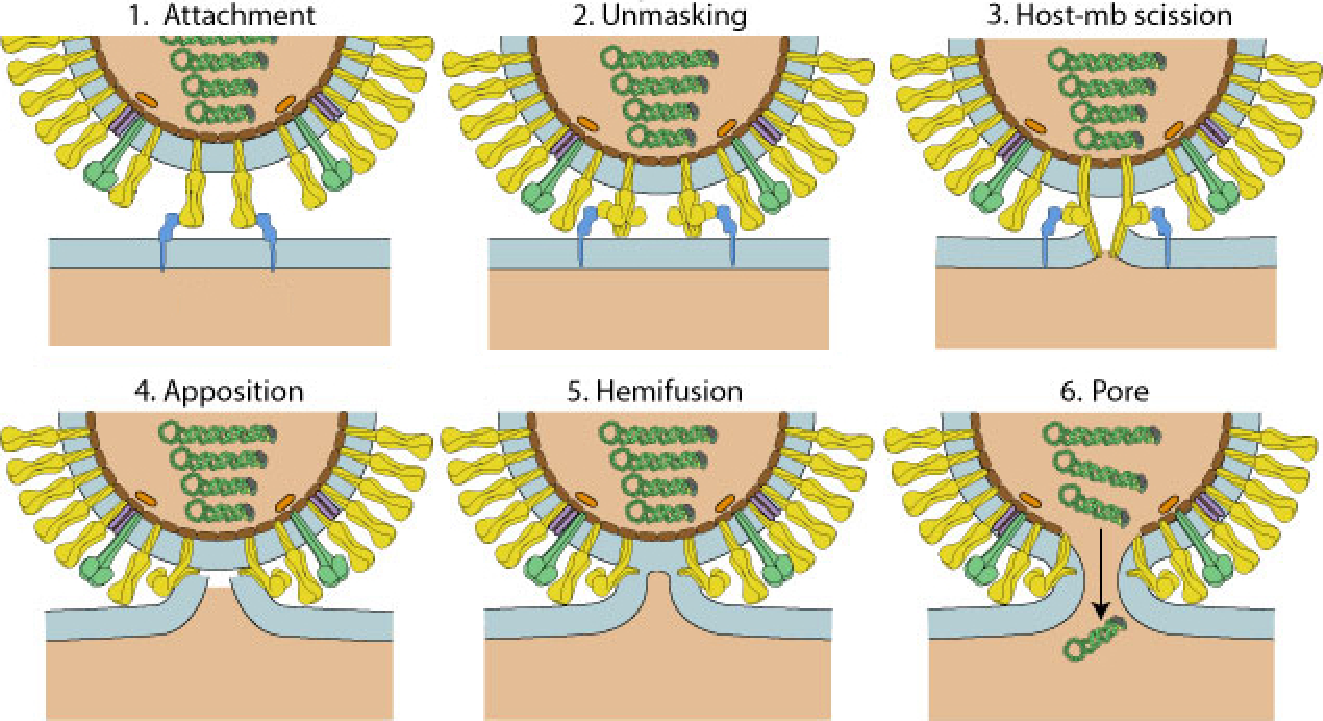
\includegraphics[width=0.95\textwidth]{virus-membrane-fusion}
  \caption[A generalized view of the steps necessary for viral--cellular membrane fusion]{A generalized view of the steps necessary for viral--cellular membrane fusion. In pre-fusion conformation, fusion proteins have their hydrophobic fusion moieties tucked away. Upon attachment (1), they are unmasked (2), interact with the target membrane and ultimately penetrate it. Conformational change in fusion proteins induces membrane scission (3) and forces the two bilayers into close proximity (4), yielding a state of hemifusion (5). Finally a fusion pore is formed (6), stabilized by the post-fusion conformation which is lower in energy than the pre-fusion state. Adapted from \cite{Hulo2011}}
  \label{fig:virus-membrane-fusion}
\end{figure}

Upon endocytic uptake, viral pathogens need to uncoat and eject their genetic material into the cytosol, as soon as their replicatory niche is reached. Escape timing is a critical issue, as late endosomes finally turn into lysosomes, capable of digesting their contents. Many enveloped viruses employ fusion mechanisms, which can be classified as type I or type II. For both types, increasing acidity associated with endosome maturation, initiates membrane fusion. Type I fusion proteins are forced into a metastable conformation prior to being added to the viral envelope and low pH triggers a conformational change to a state of lower energy. The energy released is used to force the two membranes close together resulting in their fusion (see figure \ref{fig:virus-membrane-fusion}). In type II fusion proteins, the critical transformation is not a conformational change but one in quaternary structure.

Non enveloped viruses cannot fuse with host membranes and have developed alternative approaches such as lysis (e.g. adenovirus) or ejecting their genome through pore-forming complexes (e.g. reovirus). Polyomaviruses need to pass through the \gls{er} because they rely on \gls{er} localized proteins to uncoat their capsid. For export from the \gls{er} into the cytosol, they exploit the \gls{erad} pathway, which serves as export mechanism for misfolded proteins from the endoplasmic reticulum to be degraded by proteasomes.

\renewcommand{\arraystretch}{1.5}

\begin{table}
  \label{tab:baltimore-classification}
  \centering
  \caption[The Baltimore classification scheme for viruses]{The Baltimore classification scheme is based on diversity of genetic system that have evolved in viruses. For each group, a selection of virus families capable of infecting humans, is provided, along with whether the virions are enveloped and the location of their replicatory niche. The data was obtained from \cite{Hulo2011}}
  \footnotesize
  \begin{tabular}{c|l|l|c|c}
    & Genome based class & Examples & Enveloped & Replication site \\
    \hline \multirow{4}{*}{\begin{sideways}DNA viruses\end{sideways}} &
    \multirow{2}{*}{Group I: dsDNA} &
    textit{Adenoviridae} &
    no & nucleus \\
    \cline{3-5} &
    & textit{Poxviridae} &
    yes & cytoplasm \\
    \cline{2-5} &
    \multirow{2}{*}{Group II: ssDNA(+)} &
    textit{Parvovirinae} &
    no & nucleus \\
    \cline{3-5} &
    & textit{Anelloviridae} &
    no & nucleus \\
    \hline \multirow{6}{*}{\begin{sideways}RNA viruses\end{sideways}} &   
    Group III: dsRNA &
    textit{Reoviridae} &
    no & cytoplasm \\
    \cline{2-5} &
    \multirow{3}{*}{Group IV: ssRNA(+)} &
    textit{Coronaviridae} &
    yes & cytoplasm \\
    \cline{3-5} &
    & textit{Picornaviridae} &
    no & cytoplasm \\
    \cline{3-5} &
    & textit{Hepeviridae} &
    no & cytoplasm \\
    \cline{2-5} &
    \multirow{2}{*}{Group V: ssRNA(-)} &
    textit{Filoviridae} &
    yes & cytoplasm \\
    \cline{3-5} &
    & textit{Paramyxoviridae} &
    yes & cytoplasm \\
    \hline \multirow{2}{*}{\begin{sideways}Retro\end{sideways}} &   
    Group VI: ssRNA(+)-RT &
    textit{Orthoretrovirinae} &
    yes & nucleus \\
    \cline{2-5} &
    Group VII: dsDNA-RT &
    textit{Hepadnaviridae} &
    yes & nucleus
  \end{tabular}
\end{table}

\paragraph{Replication.}
Requirements for replication of the viral genome, possible transcription and translation vary widely among different groups of viruses. A classification system, based on the diversity of mRNA production mechanisms has been devised by \cite{Baltimore1971}. Table \ref{tab:baltimore-classification} provides examples of human viruses for each of the 7 groups, whether those viruses are enveloped and where they replicate.

\paragraph{Viral export.}

\subsection{Bacterial Entry Mechanisms}

Due to the much larger size of bacterial pathogens, endocytosis is not a feasible mechanism for entry. Phagocytosis, however can deal with particle uptake of this size magnitude. While phagocytosis is a function usually only available to macrophages, some bacteria have evolved mechanisms to induce phagocytosis in other cell types. Furthermore, species such as \textit{Mycobacterium tuberculosis} and \textit{Legionella pneumophila} targeting macrophages have to be able to escape phagosomes or deal with resisting digestion.

Two recurring patterns for inducing phagocytosis in non-phagocytic cells have been described: the zipper mechanism, found in \textit{Yersinia pseudotuberculosis} or \textit{Listeria monocytogenes} and the trigger mechanism used by \textit{Salmonella enterica} and \textit{Shigella flexneri}. Not all entry strategies can be assigned to these two classes and several additional, unrelated pathways have been described.

\begin{figure}
  \centering
  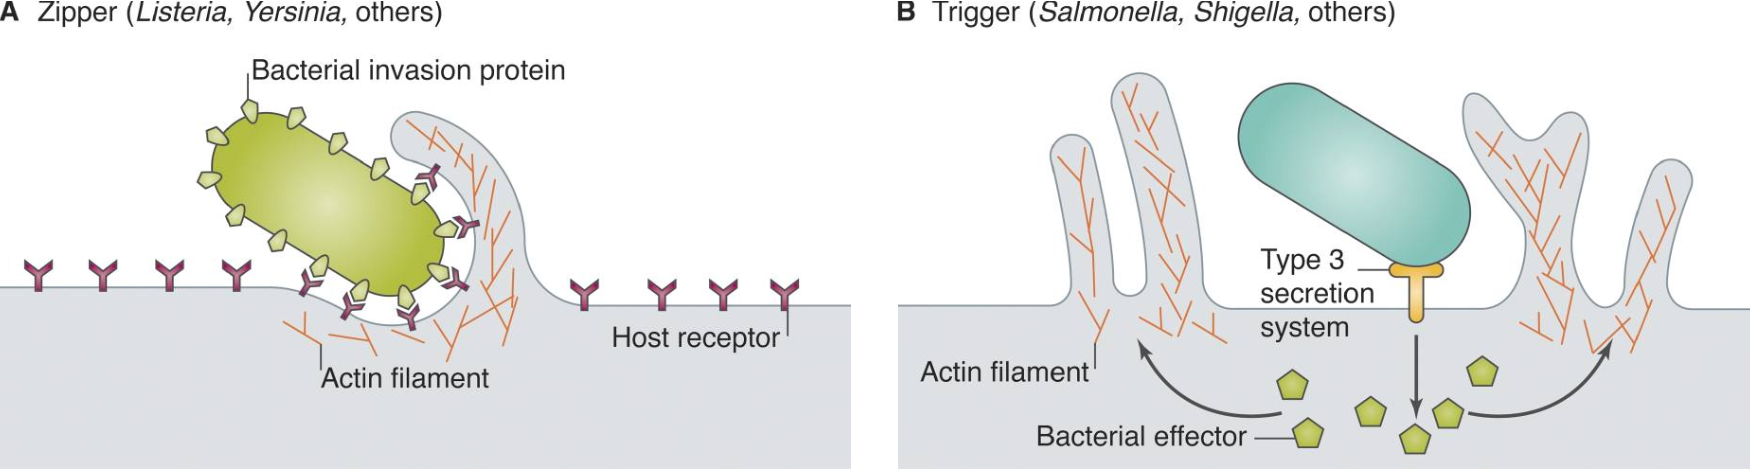
\includegraphics[width=0.95\textwidth]{zipper-trigger}
  \caption[Zipper and trigger mechanisms for bacterial host-cell entry]{Both the zipper (A) and trigger mechanisms (B) are actin dependent and lead to phagocytosis by usually non-phagocytic host cells. Zippering bacteria display an invasion protein on their surface that recruits actin filaments via a host receptor, while triggering bacteria inject an effector into the host cytosol via a type III secretion system leading to uptake. \citep{Haglund2011}}
  \label{fig:zipper-trigger}
\end{figure}

\phantomsection
\label{zipper-mechanism}

\paragraph{Zipper Mechanism.}
The first step for zippering bacteria is binding to target cell receptors by expressing adhesins. \textit{Y. pseudotuberculosis} displays invasins on its cell surface, capable of interacting with \textbeta$_1$ integrins, while \textit{L. monocytogenes} uses internalin A, a protein that binds E-cadherin. In both settings, a downstream signaling cascade leads to actin polymerization via recruitment of an \glsrev{arp-2-3} complex and \glsrev{rac-1}, yielding a phagocytic cup.

Cadherin and integrins are usually involved in anchoring cell junctions and the host cell is fooled into thinking, a neighboring cell is initiating formation of such a junction. Responding by recruiting actin at the site of bacterial attachment to cover the surface of mistaken invasion proteins leads to engulfment and phagocytosis to the bacterium. This process incurs only modest cytoskeletal rearrangements. 

\phantomsection
\label{trigger-mechanism}

\paragraph{Trigger Mechanism.}
In case of the trigger mechanism, bacterial \gls{t3ss} weakly adhere to target cell receptors (CD44 for \textit{Shigella}) and effector molecules are injected into the host cytosol through a pore formed by \glsrev{sip} or \glsrev{ipa} proteins. These induce major actin rearrangements that result in localized ruffling of the plasma membrane and subsequent swallowing of the bacterium.

Early in \textit{Shigella} entry, VirA, secreted through the \gls{t3ss} causes local destabilization of microtubules by binding to \textalpha/\textbeta-tubulin heterodimers. This in turn stimulates \glsrev{rac-1} activity, \glsrev{cdc-42} recruitment and subsequent \gls{arp-2-3} activation leading to protrusions formed by actin filaments. \Gls{ipa}C recruits the Src tyrosine kinase further enhancing actin dynamics. Upon closing of the phagocytic pocket, the \gls{t3ss}-secreted protein \gls{ipa}A binds to vinculin and induces actin depolymerization.

\textit{Salmonella} inject the proteins \glsrev{sop}E and \glsrev{spt-p}, an activator/inhibitor pair for the GTPase complex \gls{rac-1}/\gls{cdc-42}, into the host cell. First, \gls{gef} activity of \gls{sop}E induces massive actin-rearrangements leading to membrane ruffling and facilitating phagocytosis, followed by GAP activity of \gls{spt-p}, restoring the inactive \gls{gdp} state of \gls{rac-1}/\gls{cdc-42} and leading to actin depolymerization. \Gls{sop}E is degraded more rapidly than \gls{spt-p}, enabling the invading pathogen to reversibly control the pathways exploited for entering.

\paragraph{Other Entry Pathways.}
In addition to trigger and zipper type uptake, other atypical mechanisms exist. Host cell entry of \textit{Brucella abortus}, for example, has been described as invasome mediated \citep{Dehio2005}. In this actin dependent process, bacteria aggregate on the cell surface and trigger their engulfment by injecting bacterial effectors into the host via \gls{t4ss}. The internalized structure is called an invasome. Actin-independent uptake albeit rare, is possible as evidenced by \textit{Campylobacter jejuni}, which have evolved a microtubule dependent invasion strategy \citep{Kopecko2001}.

\subsection{Actin-based Intracellular Motility}
\label{subsec:actin-motility}

\section{Select Bacterial Pathogens}

A total of 5 bacterial pathogens were selected for study within the InfectX RTD project by SystemsX. This section shortly describes each organism in terms of microbiological features, pathogenesis, epidemiology and diseases caused in humans. For each organism, a chapter of \cite{Rolain2006} serves as basis and is augmented by one or two review article referenced in the first paragraph of each section.

\subsection{\textit{Bartonella Henselae}}

\textit{Bartonella henselae} is a short, rod shaped, unflagellated proteobacterium, phylogenetically closely related to the genus \textit{Brucella}, presenting 94.4\% 16S rRNA gene sequence homology, compared with \textit{Brucella abortus}. The Gram-negative bacillus is a facultative anaerobic, intracellular parasite and was first described in 1992. Relatively harmless for healthy humans, infections can become life threatening in immunocompromised patients, making the species an important opportunistic pathogen \citep{Anderson1997}.

\paragraph{Diseases.}
In immunocompetent humans, infection with \textit{B. henselae} can lead to a condition known as \gls{csd}. As the name suggests, most patients report being in contact with a cat and transmission often occurs through scratches and bites. Affecting primarily children and young adults (80\% are 21 or younger), the self limiting infection typically presents itself with lymphadenopathy. Most patients remain afebrile and do not report feeling ill, with low-grade fever and malaise shown in roughly 30\% of the cases. Recovery from uncomplicated \gls{csd} usually takes 2 to 6 months and requires no specific treatment.

Possible complications include Parinaud's oculoglandular syndrome (granulomatous conjunctivitis in one eye and parotid lymphadenitis on the same side), splenomegaly and hepatic or splenic abscesses, accompanied by fever, weight loss, fatigue and malaise. In 1 to 7\% of the cases, the disease spreads to the central nervous system, leading to encephalopathy, but recovery is usually rapid (within several weeks).

Infections with \textit{B. henselae} tend to have more severe consequences for immunocompromised patients, such as bacillary angiomatosis, bacteremia and endocarditis. \Gls{aids} patients suffering from \gls{csd} usually experience severe, progressive disease with infection spreading systematically and without appropriate treatement, fatal outcome. \textit{Bartonella spp.} are the only prokaryotes known to be able to induce angiogenic tumors such as bacillary angiomas, which may involve skin, respiratory or gastrointestinal epithelia, hart, liver, spleen, bone marrow, muscles, or lymph nodes. Bacteremia may lead to inflamed heart valves, usually requiring endocarditic patients to have heart valve replacement surgery.

\paragraph{Pathogenesis.}
\textit{B. henselae} are capable of intracellular growth in both epithelial cells, and erythrocytes. Bundle forming type IV pili are essential for binding to target cells, making them important virulence factors. Internalization into red blood cells may be spectrin mediated and the bacterial protein deformin may also be involved. Endothelial receptors involved include \gls{icam-1} uptake is either via endocytosis or by a unique cellular structure termed an invasome.

Vasculogenesis is induced though an increased production in \gls{vegf} by infected host cells. Currently it is poorly understood how the pathogen provokes overexpression but the mechanism has been determined to be protease sensitive.

\paragraph{Epidemiology.}
The role of cats and in particular kittens, as reservoirs to \textit{B. henselae} has been firmly estabished. Infected felines are asymptomatic and show no signs of illness. Cat fleas (\textit{Ctenocephalides felis}) serve as vectors to spread the bacteria among cats and have also been suspected of infecting humans. The main path of transmission to humans however, is through scratches and bites by infected cats. \textit{B. henselae} has also been found in ticks and tick bites prior to contraction of \gls{csd} have been reported.

In the United States, 24000 cases of \gls{csd} are reported yearly, yielding 2000 hospital admissions with an estimated health care cost of \$12 million. Children are more likely to be affected (80\%) and incidence is higher in males (60\%). The seasonal pattern (occurrences higher in fall/winter) is attributed to cat mating patterns, as well as pet acquisition fluctuations.

\subsection{\textit{Brucella Abortus}}

The Danish physician David Bang first isolated \textit{Brucella abortus} in 1895 from cyetic cattle tissue, investigating a contagious disease causing abortions in cows. \textit{B. abortus} are small, unflagellated proteobacteria with a cell wall consisting of an outer layer of \gls{lps} (9 nm) and an inner layer of muramyl mucopeptide complexes (3--5 nm). The Gram-negative cocobacilli appear to have evolved from free-living, soil-dwelling species and are closely related to other human pathogens such as \textit{Bartonella} spp., based on 16S rRNA sequences. Brucella species were investigated for possible use as warfare agents in the mid 20th century by several armed forces. \citep{Atluri2011}

\paragraph{Diseases.}
Brucellosis is a human disease caused by several pathogenic \textit{Brucella} species, most importantly \textit{B. abortus}, \textit{B. melitensis}, \textit{B. canis} and \textit{B. suis}. Onset may be acute or insidious and due to protean symptoms, diagnosis based on clinical presentation alone is difficult. The febrile disease is generalized and may involve many parts of the body, including nervous, skeletal, gastrointestinal, cardiovascular, respiratory and genitourinary systems. Furthermore, as the bacteria spread to other reservoir hosts via their reproductive systems, persistence of infection is crucial to the pathogen and it comes as no surprise that brucellosis can manifest as a chronic disease in humans too.

Fever is the most consistent sign of \textit{Brucella} infection and depending on what specific organs are affected, further symptoms include asthenia, anorexia, nausea, malaise, arthritis, hepatomegaly, splenomegaly, epididymo-orchitis in males, and pulmonary manifestations such as bronchitis or pneumonia. A rare complication (less than 2\%), albeit the most lethal, is infective endocarditis. Invasion of the nervous system occurs in less than 5\% of cases and often results in meningitis or meningoencephalitis with good prognosis under antimicrobial treatment.

\paragraph{Pathogenesis.}
Host entry happens primarily via the digestive system but is also possible through the respiratory tract or skin lesions. On the gastrointestinal route, \textit{Brucella} spp. target Peyer's patches (lymphoid nodules localized towards the end of the small intestine) and must therefore pass through acidic conditions in the stomach. This is facilitated by expression of two ureases capable of hydrolyzing urea and producing a protective bicarbonate buffering system. When entering through the respiratory system, \textit{B. abortus} target alveolar macrophages which serve as access point to the lymphatic system therefore facilitating systematic spread.

In order to persist at systemic sites, both active and passive mechanisms for evading the immune system are in place. \Gls{lps} of the outer cell wall disguises the bacteria from \glspl{tlr} and expression of two proteins containing \gls{tir-1} domains actively interferes with \gls{tlr} signaling.

Uptake by macrophages happens via phagocytosis, which is either triggered by nonopsonized bacteria through a lipid raft mediated mechanism or by opsonization. Although opsonin marked bacteria are 10-fold more likely to be ingested, the number of pathogens reaching their replicatory niche within the host cell is higher for nonopsonized bacteria. Maturation of early endosomes into lysosomes is important for successful infection as preventing acidification (through addition of bafilomycin A) or fusion with lysosomes (through suppression of the late-endosomal GTPase Rab7) interferes with bacterial replication. Nonopsonized bacteria finally become associated with rough ER and begin replication in ER derived vacuoles within the \gls{ergic}. Blocking the small GTPase Sar1 inhibits intracellular replication by preventing acquisition of \gls{cop-2} by ER-exit vesicles and the small GTPase Rab2, involved in ER--cis-Golgi traffic, is required for maximal proliferation.

Despite multiplying intra-cellularly in high numbers, host cells are kept alive and are even able to replicate despite infection. Furthermore \textit{Brucella} species are able to interfere with apoptosis, maintaining their replicatory niche, protected from immune response.

\paragraph{Epidemiology.}
Preferred natural reservoir species for \textit{B. abortus} are cattle (\textit{Bos taurus} and \textit{Bos indicus}) and almost all parts of the world are affected. The disease exists in both domestic and wild animals and is most prevalent in Mediterranean countries, North Africa, throughout the Middle East, India, Central Asia, as well as South and Central America. Zoonosis most often occurs through ingestion if unpasteurized milk products but airborne transmission is also possible, putting professionals involved in animal husbandry at risk. Vertical transmission among reservoir hosts can occur through lactation and horizontal transmission is facilitated by mating and placental discharge associated with aborted gestation. Human-to-human transmission is rare (but has been suspected to be possible via sexual intercourse), making humans dead-end hosts. As opposed to \textit{Bartonella}, immunodeficient patients do not seem to be especially susceptible towards \textit{Brucella} infections.

Worldwide, an estimated 500000 new cases of brucellosis occur annually, making it one of the most prevalent zoonoses. Although usually susceptible to combined antibiotic therapies of at least two agents (usually a tetracycline antibiotic combined with an aminoglycoside or rifampin), untreated brucellosis leads to a high degree of morbidity, leading to being classified a neglected zoonosis by the \gls{who}.

\subsection{\textit{Listeria Monocytogenes}}

The short, Gram-positive bacilli are non-sporeforming facultative anaerobes, capable of growing in a wide temperature range (0--50\si{\degree}C) and in many different environments. Flagellation is temperature dependent with flagellin being expressed and assembled into peritrichous flagella around 20--25\si{\degree}C but not at 37\si{\degree}C. First described in 1924 by Murray after isolation from lymph glands of diseased laboratory animals, the pathogen was found to also infect humans four years later. For much of the time since, listeriosis was considered a rare zoonotic disease and did not receive much attention. It was not until the 1980s, when several food-borne listeria outbreaks caused a shift in interest towards the pathogen, which has since become a well studied facultatively intracellular parasite \citep{Farber1991}.

\paragraph{Diseases.}
Maternal and neonatal listeriosis accounts for almost half of all infections. Listeriosis in pregnancy typically manifests in bacteraemia and presents as a self-limiting febrile disease with flu-like symptoms. Many cases, however are asymptomatic and the first sign of infection is abortion or neonatal listeriosis. Maternal infection does not necessarily carry over to the fetus, especially if proper chemotherapy is administered. Perinatal incidences are divided into early and late onset (\textgreater 5 days after parturition), with former cases typically resulting in septicemia and latter cases in meningitis. While in early onset cases the predominant route of transmission is transplacental, the situation is less clear in late onset cases. Both the maternal genital tract during child birth and environmental sources have been implicated. Despite antibiotic treatment, overall mortality rates of 30--40\% are typical and prognosis for early onset disease is worse, as it is often associated with preterm birth and advanced stage of infection. 

Among adults, most cases of listeriosis occur in T-cell deficient individuals. HIV infection, for example, increases incidence 150--300 fold compared to general population control groups. Predisposing conditions include lymphoreticular neoplasms, deliberate immunosuppression (e.g. antirejection treatment after organ transplants), alcoholism and diabetes mellitus. Despite increased susceptibility caused by immunodeficiency, roughly 30\% of all infections affect immunocompetent individuals. In healthy adults, consumption of food contaminated with \textit{L. Monocytogenes} can either lead to self-limiting febrile gastroenteritis with short incubation time (\textless 24 h) or invasive listeriosis with much longer incubation periods (3--4 weeks). The systemic form of infection often manifests as bacteraemia or as a neurological infection, but can also involve endocarditis and spread to other parts of the body. Central nervous system involvement occurs in as much as 75\% of cases and either presents as meningitis or encephalitis. Mortality rates of 35--45\%  have been reported for listeriosis in adults.

\paragraph{Pathogenesis.}
The predominant entry path for \textit{L. Monocytogenes} into the human body is via the gastrointestinal tract, where Peyer's patches are targeted. The bacteria can induce cellular uptake (see section \ref{zipper-mechanism}), even by non-phagocytic host cells via expression of cell-surface associated interanlins. Upon cell entry, the phagosomal membrane is lysed, mediated by haemolysin secretion, and actin polymerization (see section \ref{subsec:actin-motility}) provides means of intracellular movement. Listerial haemolysin (listeriolysin) is acid activated with an optimum around pH 5.5, which is reached in late endosomes and membrane lysis is caused by the formation of large transmembrane pores. Growth and replication occur in the cytoplasm and adjacent cells can be entered by pushing against the plasma membrane and forming a pseudopod-like structure which in turn is taken up the neighbor. The resulting double-membrane vacuole can be escaped by cytolysis.

In an extracellular setting, haemolysins serve to rupture erythrocytes in order to generate free iron, a limiting growth factor. Furthermore the nonspecific immune system has to be evaded and haemolysins have also been shown to be cytotoxic towards leukocytes. Additionally, expression of bacterial superoxide dismutase mitigates the effect of free superoxide radicals which play an important role in killing phagocytized bacteria.

\paragraph{Epidemiology.}
Incidence of listeriosis has initially been increasing since its recognition as food-borne disease but effects of awareness and diagnostic methods are unclear. While typically long incubation periods do pose difficulties for clinical diagnosis, the number of susceptible individuals is on the rise and certain aspects modern processing and handling of foods may be beneficial for growth of \textit{L. Monocytogenes}. Disease rates of 2--15 cases per million population per year have been reported and listeriosis is among the leading case of lethal food-borne pathogen infections. Most recent data, however suggests, that incidence is decreasing again.

Due to its non-fastidious lifestyle, \textit{L. Monocytogenes} has been isolated from a wire array of ecological niches, including soil, sewage and water (both fresh water bodies and estuaries). High persistence (up to 4 years) in soil samples is problematic when contaminated manure is used as fertilizer and biofilm formation poses challenges for eradication from food processing plants. Additionally, the ability to grow in refrigerated foods and resistance towards heat treatment such as pasteurization warrant alertness and special preventive care. Many different foods have been implicated in listeriosis outbreaks, including vegetables (potatoes, radishes and celery), seafood (shrimp, crabmeat and smoked fish), diary products (soft cheese, pasteurized and unpasteurized milk) and meats (poultry, various types of sausages and pâté).

Despite high prevalence in food (studies have found 20--80\% of meat product samples and 1--10\% of diary product samples contaminated with \textit{L. Monocytogenes}), comparatively few successful infections occur. The bacteria are ingested frequently in small doses and stool sample examinations suggest that 10-70\% of investigated populations could be intestinal carriers. While the minimum infectious dose has not been settled definitively, approximations range from $10^6$ to $10^9$ bacteria.

\subsection{\textit{Salmonella} Typhimurium}
\textit{Salmonella} are non-sporulating, Gram-negative bacilli, belonging to the family Enterobacteriaceae. The motile bacteria are able to produce peritrichous flagella and diameters span 0.7 to 1.5 \textmu m while typical lengths range from 2 to 5 \textmu m. They are closely related to the genus \textit{Escherichia}, showing only 15\% chromosomal sequence disparity. Currently, two distinct species, \textit{S. bongori} and \textit{S. enterica}, within the genus \textit{Salmonella} are recognized, both of which are pathogenic towards a wide array of hosts. \textit{S. enterica} is further divided into 6 subspecies, the most relevant of which for human and domestic animal hosts being \textit{enterica}. A large number of serovars (more than 2500) for \textit{S. enterica} subsp. \textit{enterica} have been characterized and due to an originally mistaken classification as separate species, some serovars are designated with shortened names. \textit{S.} Typhimurium, therefore is shorthand for \textit{S. enterica} subsp. \textit{enterica}, serovar Typhimurium and to emphasize that Typhimurium is not a species description it is not italicized.

The first description of the genus \textit{Salmonella} dates back to an investigation into swine fever led by Salmon and Smith in 1885. The newly isolated bacterium was wrongly proposed as the etiological agent, as the disease later tuned out to be caused by a virus \citep{Fabrega2013}.

\paragraph{Diseases.}
Two distinct disease patterns are associated with \textit{Salmonella} spp. infections, typhoid fever and salmonellosis. While the former is exclusively caused by the serovars Typhi and Paratyphi, the latter is associated with several serovars, the most frequent being Enteritidis and Typhimurium, accounting for 65\% and 12\% of cases worldwide. The current and following sections will not discuss typhoid fever.

Salmonellosis is a diarrheal disease with a short incubation period of 6--24 h, followed by nausea, vomiting, loose or liquid bowel movements, abdominal cramps and fever. Clinical features are similar to those of dysentry and other gastroenteric disease and can include bloody and mucosal stool. In most cases, the infection is self-limiting and symptoms fade away within 4 to 7 days. The most common complication is bacteraemia, which presents in 5\% of cases and is more likely to develop in children, especially if malnourished, and immunocompromised individuals. Further manifestations of invasive infections include meningitis, osteomyelitis, cholangitis, pneumonia and endocarditis. While mortality in immonocompetent hosts in developed countries is as low as 0.1\%, it can increase to 77\% for \gls{hiv} positive patients in undeveloped countries.

\paragraph{Pathogenesis.}
In order to reach the small intestine, ingested \textit{S.} Typhimurium first are exposed to the hostile environment of the stomach. A set of proteins, summarized as \gls{atr} helps mediate the acidic conditions and improves survival rates. The reamining bacteria subsequently reacht the small bowel and target its epithelial cells, with preference towards \gls{m-cells}. Flagellar motility enables penetration of intestinal mucus secretions and improves the chance of reaching the intestinal walls where adhesion can be established. Fimbriae are important attachment factors, capable of interaction with host-cell laminin and fibronectin and provide an initial platform for pathogen induced phagocytosis via trigger mechanism (see section \ref{trigger-mechanism}). 

\textit{S.} Typhimurium utilize two separate \gls{t3ss} systems for host-cell colonization, the first of which (\gls{t3ss}-1) mediates invasion. In addition to strengthening initial interactions attaching the pathogen to its target, the needle like structure serves as delivery mechanisms, capable of injecting effector proteins, including \gls{sop}E, \gls{sop}E2, \gls{sop}B (also known as SigD) and \gls{sip}A. \Gls{sop}E serves as \gls{gef} and activates \gls{rac-1} and \gls{cdc-42} via \acrshort{gdp}/\acrshort{gtp} exchange, which in turn initiate cytoskeletal rearrangements. \Gls{sop}E2 is a further \gls{gef}, highly homologous to \gls{sop}E and it is assumed to fill in for \gls{sop}E in \textit{Salmonella} strains missing the \gls{sop}E gene. \Gls{sop}B is a phosphatase, capable of hydrolyzing various substrates, including \gls{i13456p5}, which has been linked to intestinal fluid secretion causing diarrhea and \gls{pi45p2}, which is involved with membrane rigidity. Finally, the actin binding protein \gls{sip}A  stimulates stimulates actin polymerization and promotes membrane ruffling.

Upon engulfment, maturation of the phagosome and fusion with lysosomes have to be prevented. Unlike other pathogens that escape the digestive mechanisms of phagocytic vesicles by moving to the cytosol, \textit{Salmonella} replicate inside phagosome-derived \glspl{scv}. In this setting, the second translocation complex (\gls{t3ss}-2) is activated, and used to secrete effectors, including SsaB and SifA, capable of interacting with vesicular trafficking mechanisms and guiding the \gls{scv} away from its original degradation pathway. Furthermore \gls{t3ss}-2 translocated effectors induce actin polymerization events, which guide the \gls{scv} toward a perinuclear position. A last step in creating the intracellular niche needed for replication, is formation of \glspl{sif}, extending outwards from the \gls{scv}. \Gls{t3ss}-2 secretes effectors such as SifA, PipB2, SseF and SseG, which mediate the microtubule dependent processes by bundling and accumulating microtubules and regulating microtubule motor function.

\paragraph{Epidemiology.}
The global disease burden caused by nontyphoidal salmonellosis is estimated at 90 million cases per year and 150000 deaths. Incidence rates are highest in East and Southeast Asia (up to 4000 cases per 100000 population per year) and both developed and undeveloped countries are affected (incidence rates in Africa are estimated at 320 while estimates for Europe are around 690 cases per 100000 population per year). An estimated 80.3 million or 86\% of reported cases are food borne \citep{Majowicz2010}.

In order to control \textit{Salmonella} outbreaks, preventive measures in food production and processing is of major importance. This starts with disease containment in domestic animals, such as vaccination of chickens, enforcing  hygiene standards in manufacturing and distribution facilities and ends with proper preparation, exploiting heat sensitivity of the organisms. As the main route of transmission is fecal--oral, good sanitary infrastructure, treatment of sewage and water processing are crucial prerequisites in combating outbreaks of salmonellosis.
% minimum infectious dose + biofilm formation leading to asymptomatic presistence

\subsection{\textit{Shigella Flexneri}}
Shigellae are small, non-sporeforming, Gram-negative bacilli and belong to the family \textit{Enterobacteriaceae}, along with \textit{Escherichia}, \textit{Salmonella} and \textit{Yersinia}. While flagellar genes are present and their expression is observed under certain conditions, the bacteria are usually described as non-motile and unflagellated. The facultative intracellular parasite shows strong specificity towards human hosts where it typically infects the lower gastrointestinal tract.

\textit{Shigella dysenteriae} was identified as the etiological agent of dysentery by Shiga in 1897 during an epidemic in Japan with 91000 reported cases and a \textgreater 20\% mortality rate. \textit{S. Flexneri} was first described by Flexner in 1900, while investigating diseases endemic to the Philippines. Recent genetic studies suggest, that \textit{Shigella} spp. belong to the species \textit{Escherichia coli}, rather than forming a distinct genus, as only marginal sequence divergence (1.5\%) between \textit{E. coli} and \textit{S. Flexneri} was found \citep{Schroeder2008}.

\paragraph{Diseases.}
Bacillary dysentery is an acute infection of the intestine. Mild cases of the disease are self-limiting and afebrile with diarrhea and possibly vomiting as the only symptoms. In as little as 24 hours after onset, bowel movements usually begin to normalize and the condition is resolved within a few days. More severe cases are accompanied by strong abdominal cramps, fever and watery diarrhea containing blood and mucus, indicative of injury to the intestinal epithelium. While still usually self limiting in healthy individuals, recovery takes 10--14 days and relapses are possible. In immunocompromised patients, young children, especially if malnourished, and elderly individuals, life threatening complications including bacteraemia, renal failure, intestinal perforation and toxic megacolon are more frequent. Involvement of the central nervous system and respiratory tract is rare.

Administration of antibiotics is not recommended in mild to moderate cases as the disease can usually be overcome by the immune system and \gls{amr} in Shigellae is becoming an increasing concern. Oral rehydration therapy is the most effective treatment, helping the body replenish liquids and salts lost due to diarrhea. For severe infections, the use of antibiotics can become necessary and testing for resistance patterns, if possible, is advised.

\paragraph{Pathogenesis.}
Main targets of \textit{S. Flexneri} are mucosa of the distal ileum and colon where they enter epithelial cells from the basolateral side. For initial crossing over from the apical side, action of \gls{m-cells} at Peyer's patches is exploited. These specialized enterocytes constantly sample antigens from the gut lumen and pass them to intraepithelially located dendritic cells and lymphocytes. Upon uptake by basolaterally located macrophages, \textit{S. Flexneri} survive digestive action of the phagosomal vacuole by disrupting the surrounding membrane and initiating host-cell apoptosis, mediated by the bacterial effector protein \gls{ipa}B, capable of acting on a caspase 1 regulated apoptotic pathway. The bacteria are subsequently released into the sub-mucosa, where they induce phagocytosis by normal epithelial cells via trigger mechanism (see section \ref{trigger-mechanism}).

Initial contact between pathogen and target hos cell is mediated by cellular \textalpha\textsubscript{5}\textbeta\textsubscript{1} integrins and binding of \gls{ipa}B to CD44 receptors may initiate first actin rearrangements, preparing the cell for uptake. Subsequent injection of at least 6 effector proteins into the epithelial cytosol through the \gls{t3ss} triggers engulfment of the bacterium in an actin dependent process, involving the small GTPases \gls{rac-1} and \gls{cdc-42}, which recruit the actin nucleation complex \gls{arp-2-3}. \Gls{ipa}C, a component of the translocation complex, is involved in stimulating \gls{rac-1} and \gls{cdc-42} GTPase activity through an unknown mechanism and the secreted effector proteins IpgB1, IpgB2, IpgD and \gls{ipa}A facilitate actin polymerization. IpgD, an inositol phosphate phosphatase, catalyzes the hydrolysis of \acrshort{pi45p2} to \acrshort{pi5p} which promotes disassociation of cytoskeleton and membrane, increasing actin availability and making the plasma membrane more susceptibility to manipulation. The mechanism of action of IpgB2 remains to be resolved, while IpgB1 is assumed to mimic activated \glsrev{rho-g}, a small GTPase, located upstream in the signaling pathway of \gls{rac-1}. Finally, binding of \gls{ipa}A to vinculin induces depolymerization of actin, which is assumed to be important for closing of the phagocytic cup.

The resulting phagocytic vacuole has to be escaped before maturation progresses, which is accomplished in a non-acid dependent fashion, by the translocator proteins \gls{ipa}B, \gls{ipa}C and \gls{ipa}D via membrane lysis. With release into the epithelial cytosol, the replicatory niche of \textit{S. Flexneri} is reached. Actin mediated intracellular motility enables intercellular dissemination (see section \ref{subsec:actin-motility}) and targeting of epithelial tight junctions initiates break-down of the epithelial barrier, providing more pathogens with access to the basolateral side of the gut lining.

Host-cell actin utilization, is driven by activity of two bacterial proteins. VirA is secreted at the forward facing end of the rod shaped bacilli, which promotes degradation of tubulin structures and therefore clearing a path through the dense network of microtubules and surface bound \glsrev{ics}A facilitates actin polymerization at the opposite end. Both \gls{arp-2-3} and \gls{n-wasp} are involved in actin nucleation, the directed nature of which provides the driving force for locomotion.

\paragraph{Epidemiology.}
Estimates by the \gls{who} peg the disease burden caused by \textit{Shigella} spp. at 80 million annual cases worldwide, leading to 700000 deaths. Developing countries are disproportionately affected, representing 99\% of all cases, as are children less than 5 years old, accounting for 70\% of cases and 60\% of deaths. In developed countries, incidence rates of 1--2 per 100000 population are typical and Shigellae are common causes of Traveler's diarrhea.

The predominant route of transmission is fecal--oral, highlighting the importance of sanitary precautions for infection control. Proper treatment of fecal matter is important for preventing contamination of drinking water and inhibiting spreading by disease vectors such as house flies. During acute phases, diseased individuals excrete pathogens in large numbers and as few as 100--200 organisms are sufficient of causing a new infection.

\section{Select Viral Pathogens}

In addition to the previous 5 bacterial pathogens, 3 viruses were selected for study within the InfectX RTD project by SystemsX. This section shortly describes each pathogen in terms of physical features, pathogenesis, epidemiology and diseases caused in humans. For each section, a chapter of \cite{Craighead2000} serves as basis.

\subsection{Adenoviruses}
The family \textit{Adenoviridae} encompasses 5 genera of non-enveloped, medium sized (90 nm diameter) viruses, capable of infecting a broad range of vertebrate hosts. The capsid is of $T=25$ icosahedral symmetry, composed of 720 hexons arranged as 240 trimers which form the triangular facets and 12 penton capsomeres located at the vertices. A homotrimeric fiber glycoprotein protrudes from each vertex, attached to the penton base via interactions of its N-terminal domains and ending in a globular, C-terminal knob. The genome is present as double stranded DNA (Baltimore group I), is non-segmented, linear, 35--35 kb long and encodes 40 proteins.

Adenoviruses were first isolated from human adenoid tissue cultures by Rowe in 1953 and their study led to the discovery of alternative splicing in 1977, a commonly encountered phenomenon among eukaryotes. Currently, 57 serovars are recognized as pathogenic towards humans, all belong to the genus \textit{Mastadenovirus} and are classified into 6 species, labeled A through G. The following sections are mostly concerned with \textit{Human adenovirus C} \citep{Lenaerts2008}.

\paragraph{Diseases.}
In immunocompetent individuals, adenoviruses seldom cause more than transient disease with many infections even occurring subclinically and fatal outcome being very uncommon. Symptomatic cases usually manifest as respiratory tract infections or conjunctivitis and less frequently as hemorrhagic cystitis, nephritis or gastroenteritis. Infections of the oropharynx can spread to the lower respiratory tract, causing bronchitis, bronchiolitis or pneumonia, which can become chronic, leading to desquamated epithelial tissue and long-term damage to the respiratory mucosa. Heart failure and central nervous system involvement can occur in severe cases. Ocular infections range from mild, short-term follicular conjunctivitis to highly contagious keratoconjunctivitis with possible long-term damage to the cornea. \textit{Human adenovirus C} serotypes are mostly associated with respiratory diseases but have also been implicated in eye infections.

Invasive forms of disease are mostly limited to immunocompromised individuals, including transplant recipients, \gls{hiv} infected, hereditary immunodeficient and cancer patients subject to chemotherapy. In addition to the lungs, a wide variety of organs has been reported to be affected, such as partoid glands, liver, gall bladder, colon, brain and kidney and pathological changes range from perivascular cuffing to parenchymal necrosis.

\begin{figure}
  \centering
  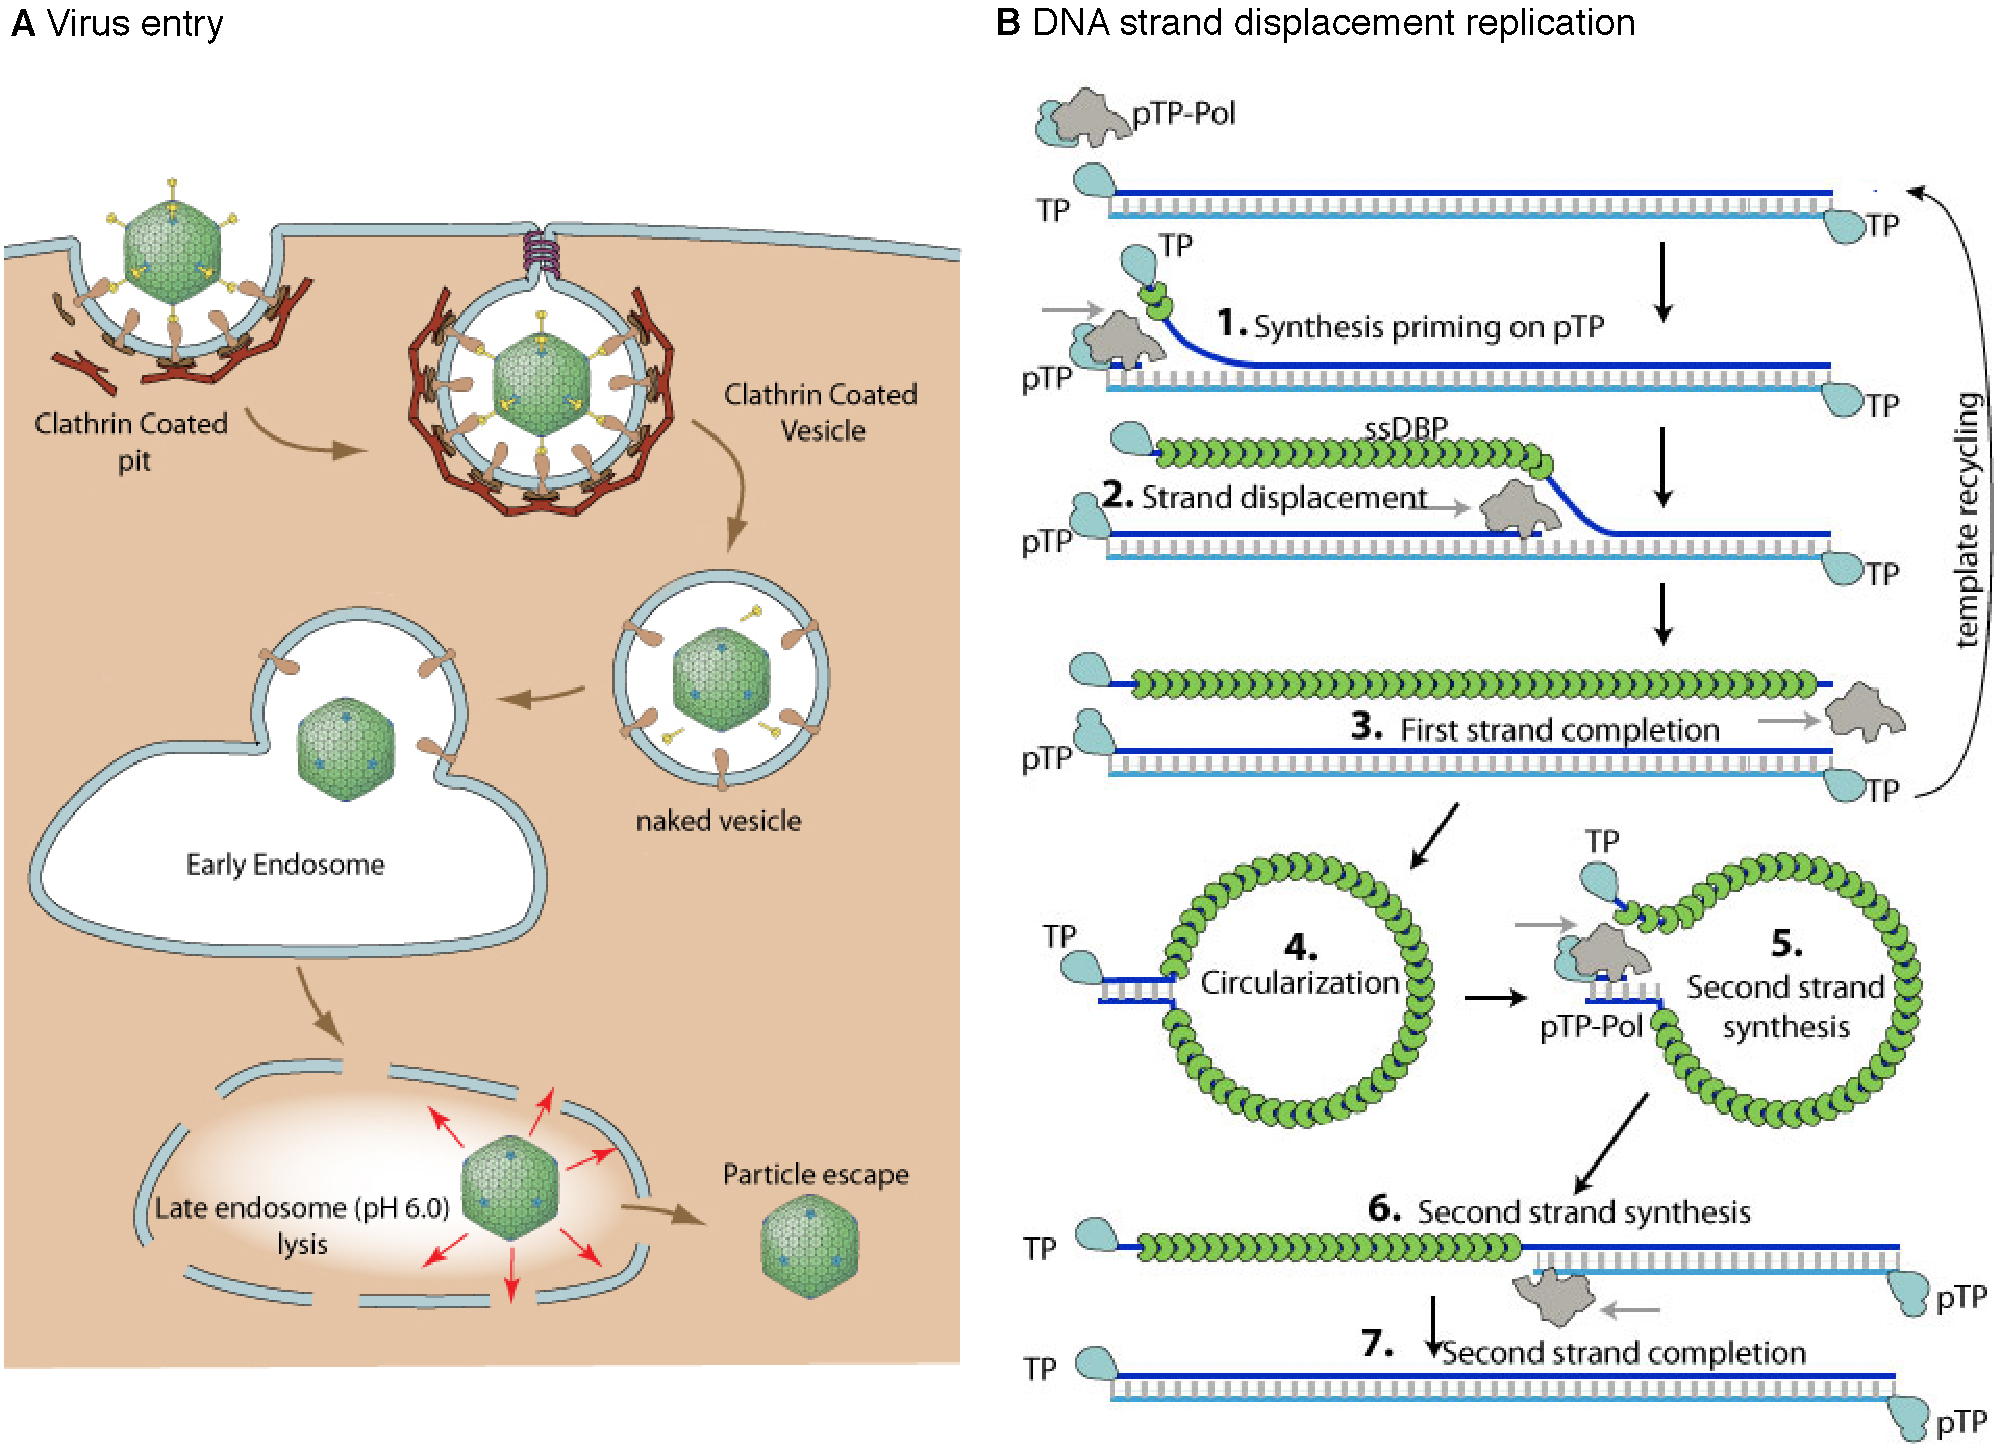
\includegraphics[width=0.95\textwidth]{adenovirus}
  \caption[Capsid structure and genome of rhinoviruses.]{Capsid proteins VP1 through VP4 form a pseudo $T=3$ icosahedral coat, roughly 30 nm in diameter around the RNA genome (A), which is monopartite, linear, 7.2 kp long and encodes 11 proteins (B). Figures adapted from \cite{Hulo2011}.}
  \label{fig:adenovirus}
\end{figure}

\paragraph{Pathogenesis.}
Initial attachment of virions is mediated by interactions between the globular knobs of viral fiber proteins and target cell \glsrevpl{car}. In \textit{Human adenovirus C} infections, cellular heparan sulfate proteoglycans serve as additional attachment factors, reinforcing adhesion. Subsequent binding of penton bases to \textalpha,\textbeta-integrin receptors induces clathrin-mediated endocytosis and leads to loss of viral fiber proteins.

The adenoviral replication cycle is divided into early, intermediate and late stages, with each seeing expression of a typical set of genes. Upon engulfment by the host cell and triggered by endosomal acidification, hexon bound protein VI disassociates from the capsid structure and induces lysis of the endosomal membrane. The remainder of the now cytosolic virion is shuttled to the nucleus by microtubular transport where viral protein IX recruits kinesin thereby procuring capsid disruption. Nuclear penetration is mediated by core protein VII and occurs at \glspl{npc}, leading to transcription of early viral genes by host RNA polymerase II. The resulting proteins manipulate various cellular processes, such as evasion of host immune response (E3), cell cycle (E1A), apoptosis (E1B and E4) and mRNA transport (E4), while also promoting viral DNA replication (E2). A virally encoded DNA polymerase replicates the genome by DNA strand displacement in a unique protein primed fashion involving \gls{ptp} acting as primer and \gls{dbp}, as well as several host proteins. With onset of replication, translation of late genes by host RNA polymerase II is initiated, leading to the production of structural proteins and proteins required for virion assembly. Encapsidation occurs in the nucleus and progeny virions are released by lysis of the host cell.

\paragraph{Epidemiology.}
Adenoviruses are endemic and ubiquitous, causing an estimated 2--5\%of all respiratory infections. Distribution is worldwide and incidence higher in the first half of the year. Children are frequently infected as serological studies show that by the age of 5 years some 50\% present antibodies towards the most common species, including \textit{Human adenovirus C}. On the order of 1 in every $10^7$ lymphoid cells in the oropharynx harbor fully assembled latent sate virions, making most humans latent carriers. Transmission can both occur via respiratory droplet or fecal-oral routes and virions are very stable towards chemical and physical agents, surviving for long periods outside their host.

Adenovirus outbreaks are a common cause of pneumonia in militaries, leading to the development of live, oral vaccines in the 1960's by the U.S. Army. The only supplier however ceased production and as of 1999, vaccinations could no longer be administered, resulting in reemerging incidence. In the first 5 years after loss of the vaccine, 110000 cases of febrile respiratory illness were reported, of which an estimated 90\% are considered preventable. By October 2011, new vaccine again was available and and has been administered to new recruits since.

\subsection{Rhinoviruses}
Investigations into the etiological agent of the common cold within the British Common Cold Research Unit led to the discovery of rhinoviruses in 1953. Initially classified as a separate genus of the family \textit{Picornaviridae}, recent genomic evidence led to a revised taxonomy, recognizing three species of rhinoviruses (A through C) as members of the genus \textit{Enterovirus}. Over 100 distinct serotypes have been isolated from humans, 74 belong to species A, 25 to B and the newly identified species C, currently under active study, may encompass an additional 55 types.

Rhinovirus virions are small (30 nm in diameter), non-enveloped, with a pseudo $T=3$ icosahedral capsid, consisting of 4 different polypeptides (VP1, VP2, VP3 and VP4) surrounding the RNA genome. There are 60 copies of each structural protein and VP1-3 face towards the outside and are responsible for antigenic diversity, while VP4 faces inwards and anchors the RNA core to the capsid. A canyon formed by VP1 and VP3 serves as receptor binding site. The viral genome consists of monopartite, linear, single stranded, positive sense RNA, roughly 7.2 kb in length and encodes a single polyprotein, which cleaved by viral proteases yields 11 proteins. Instead of a methylated 5' cap, the RNA genome is terminated by a viral protein (VPg) at its 5' end \citep{Jacobs2013}.

\paragraph{Diseases.}
Over half and up to two thirds of all cold-like illnesses are thought to be caused by rhinoviruses. In addition, asymptomatic infections, especially in children are very common with rates among children under 4 years ranging from 12 to 32\%. These surprisingly high numbers may to some extent result from virus persistence in hosts that have recovered in addition to disease that has not broken out. In adults, rates of asymptomatic carriage are significantly lower, reported at 0--2\%.

In immunocompetent individuals, symptomatic disease typically manifests as upper respiratory infection with clinical syndromes associated with common cold, including rhinorrhea, nasal congestion, sore throat, headache and possibly fever and general malaise. Disease is self-limited, incubation periods are between 12 and 72 h and within 7 to 14 days, symptoms wear off. A common complication is acute otitis media, which has been reported to happen in up to 30\% of cases in early childhood. In 41--45\% of investigated middle ear infections, rhinoviruses were detected. Further cavities that are frequently infected are the paranasal sinuses. Nose blowing has been suggested as mechanism for spreading the virus and causing rhinosinusitis.

Initially thought to primarily cause benign upper respiratory infections,  recent data clearly implicates rhinoviruses in more severe lower respiratory infections. Croup, bronchiolitis and \gls{cap} have been associated with rhinovirus infections and studies have shown that in 12, 14 and 18--26\% of respective cases, rhinoviruses were present. Furthermore, a study of children admitted to \glspl{icu} with lower respiratory tract infections detected no other pathogens in 49\% of the patients. Immunocompromised individuals are predisposed to contracting more serious forms of disease, with morbidity and mortality comparable to that of pandemic H1N1 influenza.

While not typically associated with cytopathogenic effects on epithelia of the upper respiratory tract, cell damage to lung tissue, especially among children, has been documented. Thus, rhinoviruses are linked to exacerbations of chronic pulmonary diseases such as asthma, chronic obstructive pulmonary disease and cystic fibrosis.

\begin{figure}
  \centering
  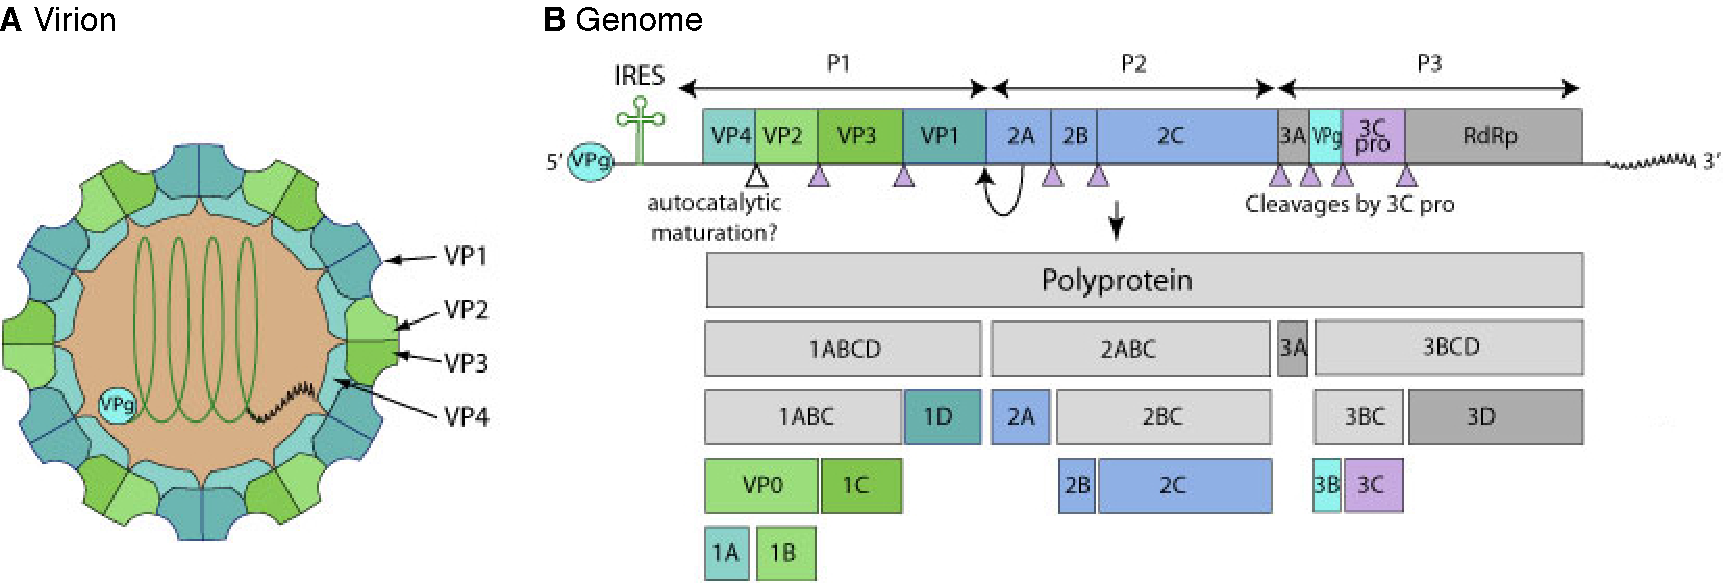
\includegraphics[width=0.95\textwidth]{rhinovirus}
  \caption[Capsid structure and genome of rhinoviruses.]{Capsid proteins VP1 through VP4 form a pseudo $T=3$ icosahedral coat, roughly 30 nm in diameter around the RNA genome (A), which is monopartite, linear, 7.2 kp long and encodes 11 proteins (B). Figures adapted from \cite{Hulo2011}.}
  \label{fig:rhinovirus}
\end{figure}

\paragraph{Pathogenesis.}
Members of rhinovirus species A and B are divided into two group according to their host cell receptors. Members of the major group form interactions with \gls{icam-1} while minor group types (including serotype 1a) associate with \glspl{vldlr}. Attachment of species C have very recently been identified as induced by \gls{cdhr3}. Upon receptor mediated endocytosis, pH dependent conformational changes in capsid structure exposes VP4 which has pore-forming properties and facilitates release of viral genomic material into the cytosol.

Host cell ribosomes readily translate the released positive-sense RNA into polyprotein, which is cleaved in \textit{cis} by 2A and 3Cpro, yielding preproteins P1, P2 and P3 (see figure \ref{fig:rhinovirus}. P1 is digested into structural capsid proteins while P2 and P3 are further processed to produce the replication machinery. Viral RNA-dependent RNA polymerase synthesizes a complementary, negative-sense RNA strand, primed by VPg, which in turn serves as template for many copies of the viral genome. These can be both translated into more protein and in a later stage of replication also be packaged into progeny virions. Final cell export is mediated by host-cell membrane lysis.

\paragraph{Epidemiology.}
Despite most infections with rhinoviruses only resulting in mild disease, economic impact both due to health care costs and loss of productivity is considerable. This is primarily owed to the overwhelming prevalence of these pathogens. Respiratory illnesses attributed to rhinoviral infections occur throughout the world and all year round with peak incidences in early fall and spring. Vaccination efforts so far have been futile, mainly because of the large number of serotypes and lack of individual epidemiological data.

Due to acid-sensitivity, fecal-oral infection is unlikely most person-to-person transmission occurs through aerosols and contact spread either direct of via fomites. Extra-host survival times of hours to days have been reported for indoor environments and up to 2 h on undisturbed skin.

\subsection{Vaccinia}
\textit{Vaccinia virus} is a species within the genus \textit{Orthopoxvirus}, alongside the exceptionally virulent \textit{Variola virus}, the etiological agent of smallpox. Immunological similarities between the two species allows for cross-protection, which coupled with the large discrepancy in pathogenicity presents a fortunate opportunity for artificially inducing acquired immunity. This was recognized by Jenner in 1798, while investigating the zoonosis of \textit{Cowpox virus} and subsequent susceptibility towards contraction of smallpox. The origins of vaccinia are unknown. It has been speculated to have derived from cowpox or smallpox, to be a hybrid of both and of being the prototype orthopoxvirus, as well as descending from an extinct ancestor.

The virions are large and brick shaped, measuring 200 by 250 by 340 nm and exist as both \gls{mv} and \gls{ev}. Structurally they are unusually complex. The linear, double-stranded DNA genome, roughly 200 kb long, is encased in an S-shaped, tube-like nucleocapsid with an outside diameter of 50 nm, a cavity of 10 nm and an overall length of 250 nm. Additionally, 47 viral proteins, of which 16 are involved in early mRNA synthesis and 28 have no known enzymatic function, are packed into a core structure. The core wall consists of two layers, the palisade (outer) layer which is 17 nm thick and an inner smooth layer, measuring 8 nm across. Centered on the top and bottom faces, two proteinaceous lateral bodies separate core from the surface membrane, forming the virion core into a biconcave disc with dumbbell shaped vertical cross sections. The lipidic surface membrane also consist of two layers, the outermost measuring 9 nm and the innermost domain is 5 nm thick. \Gls{ev} virions are additionally wrapped in a membrane derived from Golgi cisternae \citep{Marennikova2005,Condit2006}.

\paragraph{Diseases.}
While infection with variola causes severe disease manifesting in skin lesions covering the whole body, accompanied by 20--40\% mortality rates, the closely related \textit{Vaccinia virus} is far less invasive. Virulence of the latter pathogen is so low that it has been routinely used as live vaccine against the former. Owing to the massive effort put into the worldwide fight against smallpox led by the \gls{who} in the late 1960's and throughout the 1970's, the disease was found to be eliminated by 1980. At the center of the smallpox eradication program was the administration of freeze-dried, calf lymph derived vaccinia with a bifurcated needle, by multiple pricking of the skin. Towards the end of the initiative, 200 million vaccinations were performed annually.

The predominant reaction to vaccinia inoculation is localized, self-limited disease. After an incubation period of of 3--4 days, a papule with a sunken center develops at the site of infection, accompanied by erythema and swelling. Over the following days the papule increases in size and liquid begins to accumulate within. Fever may develop around days 7--10, possibly followed by malaise, headache and anorexia. Local lymphadenopathy is frequently encountered and days 8--10 typically mark the beginning of involution of the papule, which subsequently drys out and forms a scab.

Of great concern for routine vaccination procedures are complications which inevitably occur in a small numbers. Atypical side effects develop in roughly 1 per mill of cases and potentially life threatening reactions usually manifest as neurological (477.4 cases and 47.0 fatalities per 1 million) or cutaneous disease (278.4 cases and 0.2 fatalities per 1 million). Predisposing conditions for central nervous system involvement are not known and despite decades of inquiry into this pathology, it remains poorly understood. Symptoms range from febrile seizures to severe encephalitis, but so far no  neuropathological characteristics have been identified. Complications affecting the skin and mucous membranes are classified as progressive vaccinia, eczema vaccinatum and generalized vaccinia and disease severity decreases in this order. Predisposing conditions for progressive and generalized vaccinia are immunodeficiencies while a history of eczema is a risk factor for eczema vaccinatum.

\begin{figure}[t]
  \centering
  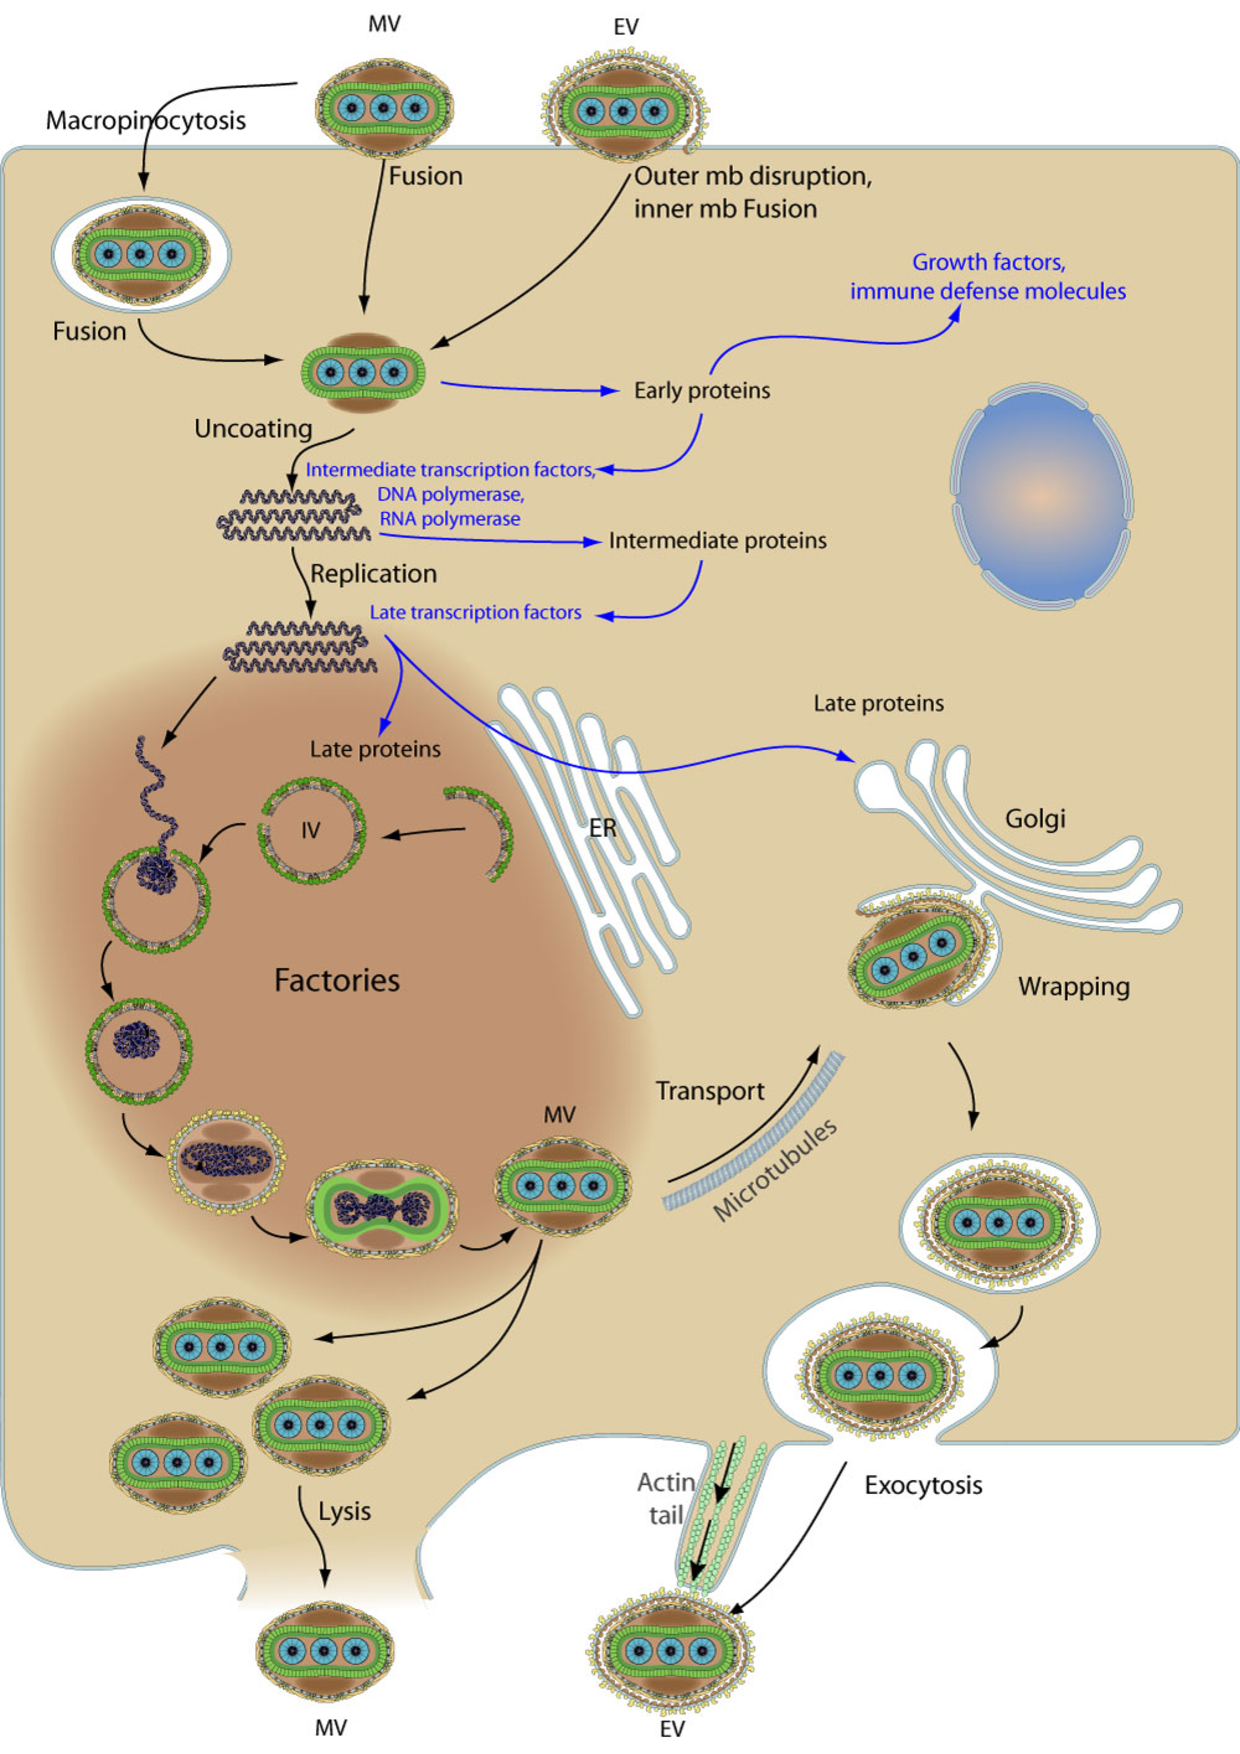
\includegraphics[width=0.75\textwidth]{vaccinia}
  \caption[Replication cycle of \textit{Vaccinia viruses} for both intracellular mature and extracellular enveloped virions.]{Capsid proteins VP1 through VP4 form a pseudo $T=3$ icosahedral coat, roughly 30 nm in diameter around the RNA genome (A), which is monopartite, linear, 7.2 kp long and encodes 11 proteins \citep{Hulo2011}.}
  \label{fig:vaccinia}
\end{figure}

\paragraph{Pathogenesis.}
Initial attachement is mediated by interaction between viral proteins and cellular heparan sulfate chains. For cell entry, various strategies have been reported, depending on the strain under investigation. WR strains induce macropinocytosis and proteins A25/A26 act as fusion suppressors that only lift their embargo under acidic conditions encountered in a maturing endosome, while other strains, such as Copenhagen, present no A25/A26 on their outer membrane and fuse directly with the target plasma membrane. Due to the additional membrane of \glspl{ev}, a differing entry mechanism needs to be emplyed. In a currently not well understood fashion, the outer membrane is lost by non-fusogenic disruption, followed by fusion of the inner virion membrane. All pathways lead to cytosolic localization of virions devoid of their envelope.

Members of the \textit{Poxviridae} family are special among Baltimore group I viruses in that their genome encodes all necessary replicatory proteins, allowing for cytosolic localization. Replication is temporally tightly regulated and consist of distinct phases of early, intermediate and late gene expression. Each class of genes encodes factors capable of initiating the succeeding stage, providing transcription level regulation. Uncoating of the core structure releases early proteins, including RNA polymerases and enzymes for mRNA processing which start transcribing early genes. At least 50 different products, such as DNA replicatory enzymes, additional RNA polymerase, mRNA processing machinery, host defense molecules and intermediate gene transcription factors, have been identified and account for 25\% of the viral coding capacity. Early gene transcripts are detectable 20 minutes after cell entry and reach their productive peak within 100 minutes of infection.

Expression of intermediate genes is initiated by accumulation of intermediate  transcription factors and the onset of DNA replication. Only 7 products of this phase are known, which functionally are mostly concerned with host defense, DNA/RNA metabolism and commencement of the final phase. Beginning 100 minutes after infection, intermediate gene transcription reaches its peak at 120 minutes and is thereafter superseded by late gene transcription, beginning 140 minutes after cell entry. Products of the final phase comprise a large number of genes (up to 75\% of the vaccinia genome) and include enzymes needed for initiating replication (RNA polymerase and modification proteins), early transcription factors and structural proteins, as well as virion assembly machinery.

DNA replication not only serves for progeny virions, but also to increase the concentration of templates used for gene expression. Both DNA synthesis and virion assembly occur within factories, readily visualized by electron microscopy as electron dense cytoplasmic inclusion bodies. Owing to the complex virion structure DNA packaging and virion assembly is an involved procedure with is incompletely understood.

\paragraph{Epidemiology.}
It is unknown if a natural reservoir of vaccinia exists It has been speculated that the virus is maintained only within research laboratories and vaccination production facilities, while others have implicated some rodent species as possible reservoir hosts. Small scale zoonotic outbreaks of vaccinia have been documented in Brazil and it was initially suspected that these were linked to vaccine that had escaped into the environment. Recent phylogenetic studies however were able to rule out this explanation but were unable to shed further light into underlying epidemiological mechanisms.

While transmission from vaccinees to unvaccinated individuals is rare, direct contact transmission is possible and such occurrences have been documented. Special care has to be taken to avoid direct contact between recently vaccinated and individuals predisposed towards developing complications.

\section{RNA Interference}
